	
%%%%%%%%%%%%%%%%%%%%%%%%%%%%%%%%%%%%%%%%%%%%%%%%%%%%%%%%%%%%%%%%%%%%%
%% This is a (brief) model paper using the achemso class
%% The document class accepts keyval options, which should include
%% the target journal and optionally the manuscript type.
%%%%%%%%%%%%%%%%%%%%%%%%%%%%%%%%%%%%%%%%%%%%%%%%%%%%%%%%%%%%%%%%%%%%%
%\documentclass[journal=jpccck,manuscript=article,layout=twocolumn]{achemso}
\documentclass[journal=jpccck,manuscript=article]{achemso}

% UHe stuff
\def\EB{E_{\rm b}}

%%%%%%%%%%%%%%%%%%%%%%%%%%%%%%%%%%%%%%%%%%%%%%%%%%%%%%%%%%%%%%%%%%%%%
%% Place any additional packages needed here.  Only include packages
%% which are essential, to avoid problems later. Do NOT use any
%% packages which require e-TeX (for example etoolbox): the e-TeX
%% extensions are not currently available on the ACS conversion
%% servers.
%%%%%%%%%%%%%%%%%%%%%%%%%%%%%%%%%%%%%%%%%%%%%%%%%%%%%%%%%%%%%%%%%%%%%
\usepackage[version=3]{mhchem} % Formula subscripts using \ce{}
\usepackage[utf8]{inputenc}
\usepackage[T1]{fontenc}
\usepackage[english]{babel}
\usepackage{braket}
\usepackage{epsfig}
\usepackage{graphicx}
\usepackage{amsmath,amsfonts,amssymb}
\usepackage{dsfont}
\usepackage{booktabs}
\usepackage{units}
\usepackage{xcolor}
\usepackage{multirow}
\usepackage{tikz,pgfplots}
\usepackage{float} %force figure position

\usetikzlibrary{patterns,shadows,trees,calc}
\usepgfplotslibrary{units}

\pgfplotsset{compat=1.8}

%%%%%%%%%%%%%%%%%%%%%%%%%%%%%%%%%%%%%%%%%%%%%%%%%%%%%%%%%%%%%%%%%%%%%
%% If issues arise when submitting your manuscript, you may want to
%% un-comment the next line.  This provides information on the
%% version of every file you have used.
%%%%%%%%%%%%%%%%%%%%%%%%%%%%%%%%%%%%%%%%%%%%%%%%%%%%%%%%%%%%%%%%%%%%%
%%\listfiles

%%%%%%%%%%%%%%%%%%%%%%%%%%%%%%%%%%%%%%%%%%%%%%%%%%%%%%%%%%%%%%%%%%%%%
%% Place any additional macros here. Please use \newcommand* where
%% possible, and avoid layout-changing macros (which are not used
%% when typesetting).
%%%%%%%%%%%%%%%%%%%%%%%%%%%%%%%%%%%%%%%%%%%%%%%%%%%%%%%%%%%%%%%%%%%%%
%\newcommand*\mycommand[1]{\texttt{\emph{#1}}}
% Define some colours
\definecolor{diplom1}{rgb}{0.0 0.4 1.0}
\definecolor{diplom2}{rgb}{0.0 0.0 0.6}
\definecolor{diplom3}{RGB}{153,0,0} %unirot

%%%%%%%%%%%%%%%%%%%%%%%%%%%%%%%%%%%%%%%%%%%%%%%%%%%%%%%%%%%%%%%%%%%%%
%% Meta-data block
%% ---------------
%% Each author should be given as a separate \author command.
%%
%% Corresponding authors should have an e-mail given after the author
%% name as an \email command. Phone and fax numbers can be given
%% using \phone and \fax, respectively; this information is optional.
%%
%% The affiliation of authors is given after the authors; each
%% \affiliation command applies to all preceding authors not already
%% assigned an affiliation.
%%
%% The affiliation takes an option argument for the short name.  This
%% will typically be something like "University of Somewhere".
%%
%% The \altaffiliation macro should be used for new address, etc.
%% On the other hand, \alsoaffiliation is used on a per author basis
%% when authors are associated with multiple institutions.
%%%%%%%%%%%%%%%%%%%%%%%%%%%%%%%%%%%%%%%%%%%%%%%%%%%%%%%%%%%%%%%%%%%%%
\author{Marko F\"orstel}
\altaffiliation{Now at: Institut für Optik und Atomare Physik, Technische Universit\"at Berlin, Hardenbergstr. 36, 10623 Berlin, Germany}
\author{Melanie Mucke}
\altaffiliation{Now at: Department of Physics and Astronomy, Uppsala University, Box 516, 75120 Uppsala, Sweden}
\author{Tiberiu Arion}
\altaffiliation{Now at: Center for Free-Electron Laser Science/DESY, Notkestr. 85, D-22607 Hamburg, Germany}
\author{Toralf Lischke}
\affiliation[IPP]{Max-Planck-Institute for Plasma Physics, Boltzmannstr. 2, D-85748 Garching, Germany}
\author{Markus Pernpointner}
\affiliation[University of Heidelberg]{Theoretical Chemistry, University of Heidelberg,
              Im Neuenheimer Feld 229, D-69120 Heidelberg, Germany}
\author{Uwe Hergenhahn}
\affiliation[IOM]{Leibniz Institute of Surface Modification, Permoserstr. 15, D-04318 Leipzig, Germany}
\alsoaffiliation[IPP HGW]{Max-Planck-Institute for Plasma Physics, Wendelsteinstr. 1, D-14791 Greifswald, Germany}
\email{uwe.hergenhahn@iom-leipzig.de}
\author{Elke Fasshauer}
\affiliation[UIT]{Centre for Theoretical and Computational Chemistry,
Department of Chemistry, University of Troms\o
-- The Arctic University of Norway, N-9037 Troms\o, Norway}
\email{elke.fasshauer@uit.no}
%\phone{+123 (0)123 4445556}
%\fax{+123 (0)123 4445557}
%\alsoaffiliation[Second University]
%{Department of Chemistry, Second University, Nearby Town}

%%%%%%%%%%%%%%%%%%%%%%%%%%%%%%%%%%%%%%%%%%%%%%%%%%%%%%%%%%%%%%%%%%%%%
%% The document title should be given as usual. Some journals require
%% a running title from the author: this should be supplied as an
%% optional argument to \title.
%%%%%%%%%%%%%%%%%%%%%%%%%%%%%%%%%%%%%%%%%%%%%%%%%%%%%%%%%%%%%%%%%%%%%
\title{Long-range Interatomic Coulombic Decay in ArXe clusters: Experiment and Theory}

%%%%%%%%%%%%%%%%%%%%%%%%%%%%%%%%%%%%%%%%%%%%%%%%%%%%%%%%%%%%%%%%%%%%%
%% Some journals require a list of abbreviations or keywords to be
%% supplied. These should be set up here, and will be printed after
%% the title and author information, if needed.
%%%%%%%%%%%%%%%%%%%%%%%%%%%%%%%%%%%%%%%%%%%%%%%%%%%%%%%%%%%%%%%%%%%%%
%\abbreviations{IR,NMR,UV}
%\keywords{American Chemical Society, \LaTeX}

%%%%%%%%%%%%%%%%%%%%%%%%%%%%%%%%%%%%%%%%%%%%%%%%%%%%%%%%%%%%%%%%%%%%%
%% The manuscript does not need to include \maketitle, which is
%% executed automatically.
%%%%%%%%%%%%%%%%%%%%%%%%%%%%%%%%%%%%%%%%%%%%%%%%%%%%%%%%%%%%%%%%%%%%%
\begin{document}

%%%%%%%%%%%%%%%%%%%%%%%%%%%%%%%%%%%%%%%%%%%%%%%%%%%%%%%%%%%%%%%%%%%%%
%% The "tocentry" environment can be used to create an entry for the
%% graphical table of contents. It is given here as some journals
%% require that it is printed as part of the abstract page. It will
%% be automatically moved as appropriate.
%%%%%%%%%%%%%%%%%%%%%%%%%%%%%%%%%%%%%%%%%%%%%%%%%%%%%%%%%%%%%%%%%%%%%
\begin{tocentry}

\begin{center}
 \includegraphics[height=3.5cm]{pics/front1.pdf}
\end{center}

%Some journals require a graphical entry for the Table of Contents.
%This should be laid out ``print ready'' so that the sizing of the
%text is correct.
%
%Inside the \texttt{tocentry} environment, the font used is Helvetica
%8\,pt, as required by \emph{Journal of the American Chemical
%Society}.
%
%The surrounding frame is 9\,cm by 3.5\,cm, which is the maximum
%permitted for  \emph{Journal of the American Chemical Society}
%graphical table of content entries. The box will not resize if the
%content is too big: instead it will overflow the edge of the box.
%
%This box and the associated title will always be printed on a
%separate page at the end of the document.

\end{tocentry}

%%%%%%%%%%%%%%%%%%%%%%%%%%%%%%%%%%%%%%%%%%%%%%%%%%%%%%%%%%%%%%%%%%%%%
%% The abstract environment will automatically gobble the contents
%% if an abstract is not used by the target journal.
%%%%%%%%%%%%%%%%%%%%%%%%%%%%%%%%%%%%%%%%%%%%%%%%%%%%%%%%%%%%%%%%%%%%%
\begin{abstract}
We report about autoionization channels of Ar inner valence ionized states in mixed ArXe clusters. 
The mixed clusters were produced by supersonic coexpansion of the two gases.
Clusters with a range of sizes and compositions were probed. 
The Xe content in the clusters was varied between 10 and 53\,\%. 
Our experimental data obtained by electron, electron coincidence spectroscopy are compared to theoretical simulations for representative cluster structures.
The combined experimental and theoretical data show that the autoionization of Ar 3s$^{-1}$ in ArXe is dominated by Interatomic Coulombic Decay (ICD) to Xe atoms in the second and higher coordination shells of the originally excited atom.
Electron Transfer Mediated Decay (ETMD3) is energetically allowed as well for
most cluster structures. It is even dominant for some of the cluster
structures, but has less intensity in the experimental spectra. We therefore
conclude that 
cluster structures with either a clear seggregation between Ar and Xe fractions, e.g. Xe core, Ar shell systems, or with few Xe atoms singled out in surface sites
are favoured.
These structures differ significantly from the majority of calculated minimum
energy structures for ArXe systems of 38 atoms, which might show that the latter structures are not realized in supersonic expansion.

We show experimentally that the relaxation of Ar inner valence states by ICD and ETMD together has an efficiency of unity, within the experimental accuracy, for all clusters expect those with the lowest Xe content.
\end{abstract}


%%%%%%%%%%%%%%%%%%%%%%%%%%%%%%%%%%%%%%%%%%%%%%%%%%%%%%%%%%%%%%%%%%%%%
%% Start the main part of the manuscript here.
%%%%%%%%%%%%%%%%%%%%%%%%%%%%%%%%%%%%%%%%%%%%%%%%%%%%%%%%%%%%%%%%%%%%%
%%%%%%%%%%%%%%%%%%%%%%%%%%%%%%%%%%%%%%%%%%%%%%%%%%%%%%%%%%%%%%%%%%%%%
%% Start the main part of the manuscript here.
%%%%%%%%%%%%%%%%%%%%%%%%%%%%%%%%%%%%%%%%%%%%%%%%%%%%%%%%%%%%%%%%%%%%%
\section{Introduction}
%
Electron spectroscopy can make important contributions to the 
research on composition and structure of free nanoparticles.\cite{
jpcc} Besides by photoionization, free electrons emerging from 
nanoparticles can also be produced by the relaxation of 
electronically excited states. One such process, which is of 
particular importance in weakly bonded systems, is the 
Interatomic or Intermolecular Coulombic Decay (ICD).\cite{
cederbaum} In ICD, an electronic excitation decays by energy 
transfer to one of its neighbour atoms or molecules, thus 
releasing a free electron from the latter site. ICD is an 
important relaxation channel e.g. for inner-valence holes in 
elements C-Ne, and also for core levels vacancies e.g. in \ce{H2O}
, where it competes with Auger decay\cite{slavicek}. 

By definition, ICD is particularly sensitive to the chemical 
environment of the atom or molecule in which the primary 
excitation has taken place. We suggest that this property of ICD 
decay spectra can be used to derive information on a nanoparticle 
or a solvation system, for example. We report here about studies 
in which we produced heterogeneous clusters of the noble gases Ar 
and Xe with different sizes, and compositions ranging from a few 
Xe dopant atoms in an Ar matrix to clusters containing an equal 
amount of both species. By the use of electron, electron 
coincidence spectroscopy and of {\it ab initio} calculations on 
prototypical systems we show how the radiationless decay spectrum 
of Ar inner valence (3s) ionized states connects to the structure 
of the clusters.

Intermolecular Coulombic Decay initially was predicted from 
theoretical considerations of the energy levels in singly vs. 
doubly ionized, and doubly vs. triply ionized, hydrogen bonded 
clusters.\cite{cederbaum} First experimental work some years 
later used Ne clusters,\cite{marburger,jahnkenedimer} but quickly 
was followed by demonstrations of ICD in a diverse range of other 
systems. Experimental and theoretical progress has been reviewed.
\cite{hergenhahn_review, averbukh_review, jahnke_review} ICD 
proceeds by an initial ionization producing an ion in an excited 
state, followed by a transfer of energy to a neighbouring site, 
and an electron emission process therefrom. In the final state a 
positive charge remains at the site of ionization, and another 
was created at another atom or molecule. Soon after, related 
autoionization processes were discovered that proceed via a 
charge transfer instead of an energy transfer. 
%These were termed `Electron Transfer Mediated Decay' 
% (ETMD),\cite{zobeley,mueller,sakai,foerstel} for transitions in 
% which the originally excited site is neutralized by the decay, 
% and 'exchange ICD' for charge transfer contributions to the 
% normal ICD amplitude.\cite{santrarev,jahnkesat}
We find that both energy and charge transfer induced 
autoionization plays a role in Ar-Xe, and will detail the 
relevant processes below. The notion of ICD requires that the 
electronic orbitals of the two sites can be distinguished, which 
typically is the case in weakly bonded systems, held together by 
hydrogen bonds or van-der-Waals bonds. In the case of strong (
covalent or metallic) bonding, there is no distinction between 
ICD and Auger decay.\cite{hergenhahn_review}

First experiments on ICD in heterogeneous systems were on Ne-Ar 
clusters.\cite{barthnear} Those were followed by studies of ICD-
like inner-shell decays in aqueous solution.\cite{
aziz,pokapanich,pokapanich2011} Pioneering work also showed the 
potential for studies of the interface between a substrate and an 
adsorbate by ICD.\cite{grieves} More detailed work on Ne-Ar 
clusters was recently presented by some of the authors.\cite{
fasshauer2014} For this system, a detailed analysis of 
photoelectron spectra with respect to structural features of the 
mixed clusters is also available.\cite{lundwall} In Ref. \citenum{
fasshauer2014} it was shown that an analysis of the ICD spectra 
allowed to decide between structural alternatives for which the 
photoelectron data were indiscriminate.

Rare gas clusters are suitable prototype systems for studies of (
e.g.) ICD, as they can easily be produced by supersonic 
expansion. Mixed rare gas clusters easily form by coexpansion of 
the two gases through a cooled nozzle. The size of the clusters 
can be changed by varying the expansion parameters, although for 
heterogeneous clusters some uncertainty remains with respect to 
the cluster size, as empirical scaling laws \cite{hagena1981} 
apply to expansion of pure gases only. Early studies of Ar-Xe 
clusters mostly focussed on the extreme cases of a single Xe atom 
embedded in an Ar cluster (e.g. Ref. \citenum{lengenprl}). 
Different sites of the dopant atom (on top of a surface, 
integrated in an Ar surface, inside the cluster) were 
distinguished by three separate bands in the fluorescence yield 
recorded as a function of excitation wavelength.\cite{lengenprl} 
Increasing the Xe concentration in the expansion lead to changes 
in the fluorescence excitation spectrum that were interpreted as 
formation of \ce{Xe2} and larger Xe complexes inside the clusters.
\cite{lengen} Experiments on Xe-rich mixed clusters were also 
conducted, and concluded that increasing the Xe content in a 
coexpanding ArXe mixture leads to the formation of Xe-core, Ar-
shell systems with a sharp interface between the two species.\cite
{tchaplyguine,hoener} This finding was confirmed by electron 
diffraction experiments.\cite{Danylchenko} Always, the observed 
Xe content in the clusters is above the Xe content in the 
expanding gas mixture, as Xe can be condensed much easier than Ar.

Most recently, on the experimental side photoelectron spectra of 
small Ar-Xe clusters were analyzed, adding to the findings in 
earlier work.\cite{Lindblad} We will discuss this paper in 
connection with our results below. Theoretical work on Ar-Xe was 
also published, and had a focus on the radiationless decay of Ar 
inner valence vacancies in these systems.\cite{fasshauer,fasshauer
_b} Interestingly, it was found that Ar 3s$^{-1}$ is stable 
against autoionization in an ArXe dimer, but is destabilized by 
adding further Xe atoms, or an Ar solvation shell, to the system. 
Again, we will detail these results in conjunction with our 
current work.

The plan of our paper is as follows: ...


%\begin{figure}
%  As well as the standard float types \texttt{table}\\
%  and \texttt{figure}, the class also recognises\\
%  \texttt{scheme}, \texttt{chart} and \texttt{graph}.
%  \caption{An example figure}
%  \label{fgr:example}
%\end{figure}

%\begin{table}
%  \caption{An example table}
%  \label{tbl:example}
%  \begin{tabular}{ll}
%    \hline
%    Header one  & Header two  \\
%    \hline
%    Entry one   & Entry two   \\
%    Entry three & Entry four  \\
%    Entry five  & Entry five  \\
%    Entry seven & Entry eight \\
%    \hline
%  \end{tabular}
%\end{table}


\section{Experimental}
%
\begin{table}
\caption{
Expansion parameters used for cluster production. Here, Xe$_{in}$ is the fraction (particle number) of Xe in the expanding gas before the expansion, $T$ the nozzle temperature, and $p$ the stagnation pressure. Experiments were done with $d = 80~\mu$m (first two sections) and $d = 100~\mu$m (bottom section) conical nozzles of 15$^\circ$ half opening angle. For the mixed clusters, $\langle N_{Ar} \rangle$ and $\langle N_{Xe} \rangle$ refer to hypothetical cluster sizes yielded with an expansion of the respective pure gas at the conditions given. These values are calculated as in ref.\ \protect\citenum{hagena1981}. Due to the much lower freezing point of Ar, we basically have an Ar seeded expansion of Xe gas. We therefore expect actual cluster sizes in-between the two limiting values given. Inaccuracies in the calculation of $\langle N\rangle$ due to fluctuations of the input parameters are less than 6\,\%. This figure does not include systematic errors of the empirical model used.
}
\label{tab:cluster}

\begin{tabular}{l c c c r r}
%
\toprule
  label  &  Xe$_{in}$ [\%]  &  $T$ [K]  &  $p$ [bar] & $\langle N_{Ar} \rangle$ & $\langle N_{Xe} \rangle$ \\
%
\midrule
% Ar, from Marko 
Ar (1)  & --- &  96.5  & 0.35  &  42  &  --- \\
% Ar, from Marko 
Ar (2)  & --- &  96.5  & 0.67  & 190  &  --- \\
% 1103 676, 679
 (a) & 1.2 &  174   & 0.32  &   4  &   62 \\
% 1103 670
 (b) & 1.2 &  174   & 0.49  &  10  &  168 \\
% 1103 671
 (c) & 1.2 &  174   & 0.68  &  21  &  362 \\
% 1103 663
 (d) & 3.0 &  172   & 0.28  &   3  &   48 \\
% 1103 640
 (e) & 5.0 &  171   & 0.51  &  12  &  202 \\
% 0506 382, Keller offset ber?cksichtigt
Xe (1)  & 100 & 183.5  & 0.68  & ---  &  517 \\     
\midrule
% 1103 653
1103, only coinc  & 3.0 &  172   & 0.51  &  11  &  196 \\
% 1103 658
  & 3.0 &  172   & 0.68  &  22  &  385 \\
% 1103 630
  & 5.0 &  167   & 0.37  &   6  &  108 \\
% 1103 629
  & 5.0 &  167   & 0.68  &  26  &  451 \\
\midrule
% 1004 867
1004, 867  & 2.5 &  154   & 2.12  &  920 & 15760\\
% 1004 868
868  & 2.5 &  158   & 1.50  &  355 &  6090\\
% 1004 886
886  & 2.5 &  161   & 2.41  &  980 & 16770\\
% 1004 858
858  & 5.0 &  149   & 2.50  & 1620 & 27700\\
%
\bottomrule
\end{tabular}
\end{table}
%
%
The apparatus used for the experiments consists of a cooled, supersonic molecular jet apparatus and a magnetic bottle spectrometer, which detects photoelectrons and secondary electrons produced after ionization with synchrotron radiation. A detailed description can be found in Ref. \citenum{arion}, and here we focus on those details specific for the current experiment. Commercial Ar and Xe gas was used. Separate containers for the two gases were filled up to pressures suitable for producing a certain mixing ratio. The gases were then allowed to mix before the expansion. Expansion parameters and mean cluster sizes according to an empirical model are given in Tab.\ \ref{tab:cluster}. We note that currently no such empirical model for heterogeneous expansions exists. We therefore can only give the mean size for a pure jet of one or the other gas at the given conditions. 

The expansion chamber for the supersonic is separated from the interaction chamber by a non-magnetic, conical skimmer with a diameter 1~mm opening (Beam Dynamics). At few cm distance behind the skimmer, the cluster jet was crossed by synchrotron radiation from the BESSY electron storage ring at Helmholtz-Zentrum Berlin. Electrons were detected by a short 'magnetic bottle� time-of-flight spectrometer, that has been described earlier.\cite{mucke_review} Experiments were carried out at the TGM-4 (last section in Tab.\ \ref{tab:cluster}) and the UE112-PGM-1 (first two sections) beamlines with linearly, horizontally polarized radiation.


\section{Theoretical Approach}

\begin{align}
 \Gamma_{ICD}  &= \sum\limits_{i,\beta} N_{ICD,i}  \Gamma_{ICD,i,\beta}\\
 \Gamma_{ETMD} &= \sum\limits_{j,\beta} N_{ETMD,j} \Gamma_{ETMD,j,\beta}\\
\end{align}

$N_{ICD} = N_{in} \cdot N_{fin} = N_{Ar} \cdot N_{Xe}
 = \sum\limits_i N_{ICD,i}$
$N_{ETMD} = N_{in} \cdot N_{fin} (N_{fin} - 1) = N_{Ar} \cdot N_{Xe} (N_{Xe} - 1)
 = \sum\limits_j N_{ETMD,j}$

$N_{ICD,i}$ and $N_{ETMD,j}$ depend on the structure

\begin{equation}
 \Gamma_{\beta}(E_{res}) = 2\pi \left|
                           \braket{\Phi_{in}| H_f |\chi_{\beta}}
                           \right|^2
\end{equation}

\begin{equation}
 \Gamma_{ICD,i,\beta} = 2\pi
                        \frac{\sigma^{(X_E)}(\omega_{vp,\beta})}
                        {R_i^6 \, \omega_{vp,\beta}^4 \tau_{in,\beta}}
\end{equation}


\begin{equation}
 \Gamma_{ETMD,j,\beta} = 2\pi \sum\limits_{m,M_{in}',D}
                        \frac{a_m \Theta_m(\alpha_i) \sigma^{(X_E)}(\omega_{vp,\beta})
                              \tilde{D}_{m,j,\beta}(M_{in,D},M_{in,D'})}
                         {R_j^6 \omega_{vp,\beta}}
\end{equation}


\begin{equation}
\end{equation}


\begin{equation}
\end{equation}


\begin{equation}
\end{equation}


\begin{equation}
\end{equation}


\begin{equation}
\end{equation}



\begin{equation}
\end{equation}



\section{Cluster Structures}

\begin{figure}[h]
 \centering
 \includegraphics[width=8.5cm]{pics/cluster_2_overview.pdf}
 \caption{Cluster structures with 13 argon atoms and two additional xenon
          atoms on different surfaces of the argon icosahedron:
          \textbf{a)} closest possible \textbf{b)} middle \textbf{c)}
          furthest away.}
 \label{figure:cluster_2_overview}
\end{figure}



\begin{figure}[h]
 \centering
 \includegraphics[width=8.5cm]{pics/cluster_3_overview.pdf}
 \caption{Cluster structures based on 55 atoms icosahedral cluster structure.
          \textbf{a)} 1 xenon atom on the surface of a 55 atoms icosahedral
          argon cluster. \textbf{b)} six xenon atoms inside a 55 atoms cluster
          grouped on one side. \textbf{c)} six xenon atoms distributed
          in a 55 atoms cluster. }
 \label{figure:cluster_3_overview}
\end{figure}

\section{Theoretical Results
\label{sec:th_results}}
%
%
\begin{table}[h]
\small
\centering
\caption{Structural and calculated properties of some model clusters.
The cluster structures are characterized by the number of Ar and Xe atoms,
and are arranged in three groups according to gross structural properties. 
The first group contains Xe core-Ar shell systems of various
size and relative Xe content.
In the second group, model structures for small clusters are displayed,
in which 1-2 Xe atoms are added at systematically varied locations
to an icosahedric Ar clusters consisting of one or two full shells,
or in which 1-6 Ar atoms of such cluster were replaced by Xe atoms.
The last group contains data for calculated minimal energy structures
of mixed ArXe clusters.\protect\cite{marques}
The cluster structures are classified into core-shell structures (cs),
structures with seggregated xenon atoms (in) and completely mixed
structures.
The columns `ICD' and `ETMD' are the respective partial decay widths
in \unit[$10^{-4}$]{eV}, and `\% ICD' gives the percentage of ICD in
the total decay width.
See text for details.
\label{table:theo_gammas}
}
\begin{tabular}{rrrrcccccrrr}
\toprule
\# & \# Xe & \# Ar & Xe$_{\rm cl}$\% & str. cl. & pos. & rel. pos. & ICD   &  ETMD & \% ICD & Fig.\\ %$\Gamma_{\rm ICD,ETMD}$\\
\midrule
 1 &     1 &    12 &  7.7  & cs    &         &          & 0.000 & 0.000 &  -- &\\ %    0.0            \\     ArXe\_2\_1atom      
 2 &     1 &    54 &  1.8  & cs    &         &          & 0.000 & 0.000 &  -- & \ref{figure:xe_3_in}\\ %    0.0            \\     ArXe\_3\_1atom      
 3 &     2 &    53 &  3.6  & cs    &         &          & 0.033 & 0.167 &  16.7& \ref{figure:xe_3_in}\\ %2.006$\cdot 10^{-5}$ \\ ArXe\_3\_2atom      
 4 &  1415 &   642 & 68.8  & cs    &         &          & 7.039 & 2.573 &  73.2& supp.\\ %9.612$\cdot 10^{-4}$ \\ ArXe\_8\_1layer     
 5 &   561 &  3310 & 14.5  & cs    &         &          &       &       &  85  & \ref{figure:xe_6_lay5}\\ % c6l5
 
\midrule
 6 &     1 &    13 &  7.1  & cs    & surface &          & 0.792 & 0.000 & 100.0& \ref{figure:surf}\\ %7.922$\cdot 10^{-5}$ \\ XeAr\_2\_surface    
 7 &     1 &    13 &  7.1  & cs    & edge    &          & 0.013 & 0.000 & 100.0&\\ %1.320$\cdot 10^{-6}$ \\ XeAr\_2\_edge       
 8 &     1 &    13 &  7.1  & cs    & vertex  &          & 0.050 & 0.000 & 100.0&\\ %5.013$\cdot 10^{-6}$ \\ XeAr\_2\_vertex     
 9 &     2 &    13 & 13.3  & cs    &         & closest  & 0.101 & 0.151 &  40.1& \ref{figure:2tops}\\ %2.523$\cdot 10^{-5}$ \\ XeAr\_2\_2top       
10 &     2 &    13 & 13.3  & cs    &         & middle   & 0.159 & 0.008 &  95.4& \ref{figure:2tops}\\ %1.665$\cdot 10^{-5}$ \\ XeAr\_2\_2midtop    
11 &     2 &    13 & 13.3  & cs    &         & furthest & 0.159 & 0.002 &  98.9& \ref{figure:2tops}\\ %1.605$\cdot 10^{-5}$ \\ XeAr\_2\_2endtop    
12 &     1 &    55 &  1.8  & cs    & surface &          & 0.064 & 0.000 & 100.0& \ref{figure:surf}\\ %6.371$\cdot 10^{-6}$ \\ XeAr\_3\_surface    
13 &     1 &    55 &  1.8  & cs    & edge    &          & 0.048 & 0.000 & 100.0&\\ %4.791$\cdot 10^{-6}$ \\ XeAr\_3\_edge       
14 &     1 &    55 &  1.8  & cs    & vertex  &          & 0.027 & 0.000 & 100.0&\\ %2.701$\cdot 10^{-6}$ \\ XeAr\_3\_vertex     
15 &     1 &    54 &  1.8  & in    & edge    &          & 0.077 & 0.000 & 100.0&\\ %7.708$\cdot 10^{-6}$ \\ XeAr\_3\_edge\_in   
16 &     1 &    54 &  1.8  & in    & vertex  &          & 0.053 & 0.000 & 100.0&\\ %5.258$\cdot 10^{-6}$ \\ XeAr\_3\_vertex\_in 
17 &     2 &    53 &  3.6  & in    &         &          & 0.117 & 0.055 &  68.1&\\ %1.711$\cdot 10^{-5}$ \\ XeAr\_3\_2in        
18 &     6 &    49 & 10.9  & in    &         &          & 0.375 & 0.405 &  48.1& \ref{figure:ar_3_6in}\\ %7.796$\cdot 10^{-5}$ \\ XeAr\_3\_6in        
19 &     6 &    49 & 10.9  & mixed &         &          & 0.292 & 0.674 &  30.3& \ref{figure:ar_3_6in}\\ %9.660$\cdot 10^{-5}$ \\ XeAr\_3\_6\_scat    
                                                                                                 \midrule
20 &     2 &    36 &  5.3  & cs    &         &          & 0.117 & 0.151 &  43.6& supp.\\                        % Ar$_{36}$Xe$_{2}$   
21 &     4 &    34 & 10.5  & mixed &         &          & 0.248 & 0.587 &  29.7& supp.\\                        % Ar$_{34}$Xe$_{4}$   
22 &     5 &    33 & 13.2  & mixed &         &          & 0.335 & 0.844 &  28.4& supp.\\                        % Ar$_{33}$Xe$_{5}$   
23 &    13 &    25 & 34.2  & mixed &         &          & 0.828 & 5.414 &  13.3& supp.\\                        % Ar$_{25}$Xe$_{13}$  
24 &    24 &    14 & 63.2  & mixed &         &          & 1.488 &16.718 &   8.2& supp.\\                        % Ar$_{14}$Xe$_{24}$  
25 &    25 &    13 & 65.8  & in    &         &          & 1.432 & 4.995 &  22.3& supp.\\                        % Ar$_{13}$Xe$_{25}$  
26 &    35 &     3 & 92.1  & in    &         &          & 2.017 & 7.051 &  22.2& supp.\\                        % Ar$_{3}$Xe$_{35}$   
\bottomrule
\end{tabular}
\end{table}
%
The geometrical properties as well as the total ICD and ETMD decay widths
of the investigated structures are shown in Table \ref{table:theo_gammas}.
It is important to remember that the first ICD channel opens at a
channel opening distance of \unit[7.58]{\AA}. In the smallest
clusters with only one argon layer around each
xenon atom, the Ar-Xe pair distances are below that value, therefore 
no ICD can take place. Also, by definition, two Xe atoms are
required for ETMD(3), hence it cannot occur in clusters with only one xenon atom.
%Because secondary electrons are observed in the experimental spectra
%we exclude all structures without any signal from our further
%discussions.
%
\begin{figure}[H]
 \centering
 \includegraphics[width=8.0cm]{pics/surf.pdf}\\
 \includegraphics[width=8.0cm]{pics/R_comp.pdf}
 \caption{
 %
 Top panel: Simulated electron emission spectra of an Ar 3s vacancy in 
          argon clusters
          consisting of 13 and 55 atoms, with an additional xenon atom residing
          on top of one of the argon surfaces.
          Bottom panel: Distribution of Ar-Xe distances $d$ in the studied ArXe
          clusters. The ICD channels to final states involving Xe 5p$_{3/2}^{-1}$ and 
          5p$_{1/2}^{-1}$ vacancies open at \unit[7.58]{\AA} and
          \unit[36.00]{\AA}, resp.; the former distance is marked by a vertical dotted line. 
          Only pairs at longer interatomic
          distances contribute to the electron emission spectra.
          Larger Ar-Xe distances, as found in the larger cluster,
          correspond to features at higher kinetic energy of
          the ICD electron (top panel).}
 \label{figure:surf}
\end{figure}

%In the investigated structures several different aspects have to be
%taken into account which we will discuss separately if possible
%on selected structures.



We will now discuss features of several structures, using selected examples.
First we consider clusters having an argon core of 13 and 55 atoms with a single xenon
atom on one of the surfaces (see Figure \ref{figure:cluster_3_overview}a
for the 55 atoms core).
Secondary electron spectra simulated for these systems are shown in Figure \ref{figure:surf}, top panel.
%two different argon core sizes one consisting
%of 13 and one consisting of 55 atoms with one xenon atom on one of
%the surfaces (see Figure \ref{figure:cluster_3_overview} Panel a)
%for the 55 atom core). The simulated secondary electron spectra are
%shown in Figure \ref{figure:surf} Panel 1.


Because the structures have only one xenon atom, an ETMD(3) is not possible
and only ICD is to be expected. 
%Both spectra show several smaller peaks which
%are convoluted into one single peak with a maximum at
%approximately \unit[0.2]{eV}. 
%In comparison to the 13 argon atoms core
%spectrum t
The spectrum pertaining to the clusters with larger (55 atoms) Ar core shows
signals at higher energies of the secondary electron. These features
can be explained by investigating the Ar-Xe distance distributions
in the clusters, shown
in the bottom panel of Figure \ref{figure:surf}. 
Every different atom pair distance
yields in a different energy of the secondary electron and only pairs
with a distance of larger than the channel opening distance
(dashed, gray line) will contribute
to the spectrum. 
%In our model, there is a one-to-one correspondence between interatomic distance $d$ and kinetic energy of the ICD electron.
The larger the interatomic distance, the higher is the
kinetic energy of the secondary electron for a given channel.
Since the cluster with an Ar core of 55 atoms is larger, and therefore
contains Ar-Xe pairs with larger distances, its spectrum extends to
higher energies.
%energies as well.
This relation between ICD energy and cluster size holds true for all cluster structures.
%This explains why the ICD spectrum for larger clusters extends to higher energies, and holds for all cluster structures.

\begin{figure}[ht]
 \centering
 \includegraphics[width=8.5cm]{pics/2tops.pdf}
 \caption{Simulated electron emission spectra of an Ar 3s vacancy in 
          argon clusters consisting of 13
          argon atoms with two additional xenon atoms on top of two different
          argon surfaces. ICD and ETMD spectra are shown for three
          different relative positions of the two xenon atoms. If 
          the xenon atoms are close to each other, an ETMD process is
          clearly visible. In the other two cases the spectra are dominated by
          the ICD spectrum.}
 \label{figure:2tops}
\end{figure}
%
For clusters with more than one xenon atom, also ETMD(3) is possible.
Depending on the positions of the xenon atoms relative to each other and to the Ar core, the spectra are expected to be different.
As an example, we discuss clusters with a core of 13 argon atoms and two xenon atoms on different surfaces. 
Their xenon content is \unit[13.3]{\%} and thus close to the experimental one of \unit[10-12]{\%} for the lowes xenon admixture.
The cluster structures were illustrated in Figure \ref{figure:cluster_2_overview}, simulated spectra are shown in Figure \ref{figure:2tops}.
In all three cases, both ICD and ETMD(3) are energetically allowed. The ICD
spectra do not change qualitatively by adding the second xenon.
%either identical or at least very similar to the ones for
%cluster with a single  consisting of one
%convoluted peak at approximately \unit[0.2]{eV}. 
However, the ETMD(3) spectra
are very sensitive to the relative position of the two xenon atoms.
Two aspects have to be taken into account: an energy shift of the peaks due
to different charge distances in the final state (i.e. the interatomic Xe-Xe
distance) and the decrease of the decay width with $R^{-6}$, $R$ being the distance
between the electron transfer unit and the xenon atom ionized in the final state.
The larger the distance between the xenon atoms, the higher are the energies
of the secondary electrons and the smaller are the decay widths. 
Therefore, a
significant contribution from ETMD(3) compared to ICD is only
seen if the two xenon atoms reside on two adjacent
surfaces. 
%{\it Q: Ich verstehe nicht was der n\"chste Satz sagen soll.}
The three energetically separated peaks in the ETMD(3) spectrum pertain to different combinations of the Xe 5p$_j^{-1}$ vacancy states, which have a substantial fine-structure splitting (see Table \ref{tab:valence}). 
%\ref{sec:exp_results}).
%
%The threefold peak structure of the ETMD(3) peak does in contrast to
%the ICD spectrum not stem from different triple structures but from the
%four different decay channels for one triple structure.

\begin{figure}[ht]
 \centering
 \includegraphics[width=8.5cm]{pics/ar_3_6in.pdf}
 \caption{Same as Figure \protect\ref{figure:2tops}, for clusters consisting of
          55 atoms, 6 out of which are xenon atoms. These are either grouped
          on one side of the cluster (label `group') or evenly distributed
          in the cluster interior (label `scattered').}
 \label{figure:ar_3_6in}
\end{figure}
%
For the 55 atoms clusters, a xenon content of \unit[10--12]{\%}
corresponds to six xenon atoms out of a total of 55 atoms. These can form a connected 
group in one part of the cluster or can be evenly distributed,
as shown in Figures \ref{figure:cluster_3_overview}b and \ref{figure:cluster_3_overview}c. The
ICD and ETMD(3) spectra for these structures are shown in Figure \ref{figure:ar_3_6in}.

For both cases the overall ICD spectra are very similar, and show a maximum at a kinetic energy of approximately \unit[0.3]{eV}. 
In case of grouped xenon atoms, the ICD spectrum extends to slightly higher energies, corresponding to ArXe pairs at slightly larger spatial distances.
A more significant difference is observed in the ETMD(3) spectra. 
The interatomic xenon distance is shorter in clusters, in which the xenon atoms form a connected group.
Hence, the triple structure of the ETMD(3) spectrum is seen at lower kinetic energies. 
Additionally, the probability for an electron
transfer from a xenon to an argon atom decreases exponentially with the
interatomic distance. Therefore, only those xenon atoms which have direct
argon atom neighbours have a significant contribution to the
total decay width, and the total ETMD(3) decay width is lower for the structure with
grouped xenon atoms than for
the structure with evenly distributed xenon atoms (see Table \ref{table:theo_gammas}).

\begin{figure}[ht]
 \centering
 \includegraphics[width=8.5cm]{pics/xe_3_in.pdf}
 \caption{Same as Figure \protect\ref{figure:2tops}, for argon clusters with
          one or two xenon atoms in the core of the cluster (55 atoms total). 
          All ICD and ETMD channels are closed, if the cluster contains only 
          a single xenon atom. For clusters with two xenon atoms
          in the core, the first ICD channel is open for some pairs,
          and additionally ETMD is possible for multiple triples. Due to a
          different distance distribution compared to the clusters with an argon
          core (Figure \protect\ref{figure:2tops}), 
          the ICD peak is shifted to higher kinetic energies.}
 \label{figure:xe_3_in}
\end{figure}
%
For comparison with the previous assumptions of a xenon core surrounded
by argon atoms we investigated clusters of 13 and 55 atoms with one or two
xenon atoms in the core. Some of the corresponding
spectra are shown in Figure \ref{figure:xe_3_in}.

%For the clusters with only one xenon atom in the core and the ionization
%energies used for the simulation of the secondary electron energies
%all ICD channels are closed. Since the cluster contains only one xenon atom,
%an ETMD(3) is not possible. Hence there is no signal to be expected at all.
For a core consisting of two xenon atoms both an ICD and an ETMD(3) spectrum
can be seen. Compared to the cluster structures involving an argon core, the ICD peak is
shifted to higher ICD electron energies. 
Additionally, the ICD and ETMD(3) spectra overlap.
For ETMD(3), only three of the four different decay channels are
energetically allowed.

\begin{figure}[ht]
 \centering
 \includegraphics[width=8.5cm]{pics/c6l5.pdf}
 \caption{Same as Figure \protect\ref{figure:2tops},
          for a large cluster consisting
          of a xenon core of 561 atoms surrounded by five complete layers of
          argon atoms (Xe content: 14.5\,\%) for both an icosahedral and
          cuboctahedral basic structure.
          The ICD and ETMD peak overlap such, that the peak
          structure might not be visible.}
 \label{figure:xe_6_lay5}
\end{figure}
%
In the first experiments very large argon-xenon clusters of 
$\approx 4380$ atoms with a xenon content of \unit[19]{\%}
were measured,\cite{Mucke_phd}
which we in one example approximate by a cluster consisting of 561 xenon
atoms surrounded
by five layers of argon atoms (3871 atoms in total). In order to take the
better stabilization of charges in larger clusters into account, the
ionization energies of the XL clusters (see Table \ref{tab:valence})
were used.
The spectra are shown in 
Figure \ref{figure:xe_6_lay5}.

Compared to the small clusters with a xenon core in Figure \ref{figure:xe_3_in}
the ICD peak is broadened and shifted to higher ICD electron energies which is
expected due to the larger interatomic Ar-Xe distances in the large cluster and
the better stabilization of charges, which is relevant mostly for the final state, but also the initial state.
The ETMD(3) peak is shifted to slightly higher energies as well. This allows opening of the
fourth decay channel, pertaining to Xe 5p$_{1/2}^{-1}$ Ar 3p$_{1/2}^{-1}$ final states.

We also note that the percentage of decay via ICD is practically
independent of the Xe content for large clusters with a core-shell structure.
This can be expected, as both decay processes are most pronounced for the
atoms in the interface region of the xenon core and the argon shell.
The ETMD(3), depending on the electron transfer from one xenon atom to the
initially ionized argon atom and hence the corresponding orbital overlap,
is a pure interface effect involving the argon atoms with direct xenon
neighbours and the two xenon layers closest to the argon shell.
The ICD has a stronger long range character, due to which the description
of decays with partners of at least twice the smallest channel opening
distance is necessary for clusters. However, the bigger the clusters are,
the more homogeneous does the interface region become for clusters of
different sizes. This manifests itself in the distribution of relevant
Ar-Xe pair distances (compare Fig. \ref{figure:surf} lower panel).
As a consequence, the ICD spectra of two large clusters of different size
do hardly differ.


\section{Experimental Results}
\label{sec:exp_results}
%
%
\begin{table}
\caption{Properties of the outer valence spectra of mixed ArXe clusters. 
Spectra of pure Ar and Xe clusters are included for reference. 
All spectra were recorded at $h\nu = 17$~eV, except for the pure Xe clusters ($h\nu = 60$~eV). 
Binding energies $\EB$ were determined as the centre of gravity of the respective feature, while band width $w$ are the FWHM of a Gaussian fit. 
The average Xe content of the cluster ensemble, Xe$_{\rm cl}$, was determined from the areas of the respective photolines, corrected by their atomic photoionization cross sections (Ar 33.0 Mb, Xe 51.3 Mb)\cite{samson2002}.
Uncertainties are estimated as $\pm$3\,\% for the Xe content and 0.05~eV for the binding energies. 
The row labelled `(th.)' gives the binding energies used in the simulations of this paper, and the last row their atomic counterparts. 
Values for Ar 3p in the last row refer to the fine structure states.
\label{tab:valence}}
\begin{tabular}{ l c c c c c c c c}
%
\toprule
 \multicolumn{2}{r}{size} &  Xe$_{\rm in}$& $\EB$ (eV)& $w$ (eV)& \multicolumn{2}{c}{$\EB$ (eV)}  & $w$ (eV) &  Xe$_{\rm cl}$ \\
%
 \multicolumn{2}{r}{(label)}&  (\%) & Ar 3p & Ar 3p & Xe 5p$_{1/2}$ &  Xe 5p$_{3/2}$ & Xe 5p$_{3/2}$  &  (\%) \\
\midrule
% Ar, from Marko
 Ar & (1) &&  15.3  &  1.1 & & & &  \\
% Ar, from Marko 
 Ar & (2) &&  15.1  &  1.3 & & & &  \\
%
%  columns in the following: energies c.g. 51-plt-oval, widths Marko Diss., Xe content Marko Diss
% 1103 676, 679
 ArXe & S &1.2 & 15.36 & 0.9 & 13.07 & 11.75 & 0.85 & 12\\
% 1103 670
 ArXe & M &1.2 & 15.30 & 1.0 & 12.97 & 11.61 & 0.85 & 11\\
% 1103 671
 ArXe & L &1.2 & 15.25 & 1.1 & 12.91 & 11.52 & 1.08 & 10\\
% 1103 663
 ArXe & S &3.0 & 15.39 & 0.8 & 13.06 & 11.68 & 1.02 & 29\\
% 1103 640
 ArXe & M &5.0 & 15.31 & 0.6 & 12.96 & 11.44 & 1.24 & 53\\
% 0506 
 Xe &  & & & & 12.76 & 11.19 & 1.18 & 100\\
%
\midrule
%
%  1004  886  (UHe, c.g. + roi values)
 ArXe & XL &2.5 & 15.15 & 1.3 & 12.59 & 11.01 & 1.24 & 19\\
%
\midrule
% Date: Wed, 20 Jan 2016 11:27:39, From: Elke Fa?hauer <elke.fasshauer@uit.no>
 Ar, Xe & (th.) && 15.3 && 13.0 & 11.5 &&\\
%
 \multicolumn{2}{l}{(atomic)\cite{velchev,sansonetti}} && 15.76|15.94 && 13.43 & 12.13 &&\\
%
\bottomrule
\end{tabular}
\end{table}

\subsection{Outer valence spectra}
%
This section describes and discusses the outer valence spectra of the mixed
Ar-Xe clusters. The main information we obtain from these spectra within
the context of our theoretical considerations are the single ionization
potentials and the relative Xe
contents in the mixed clusters (see Table\ \ref{tab:valence}). 
%
\begin{figure}[ht]
 \centering
 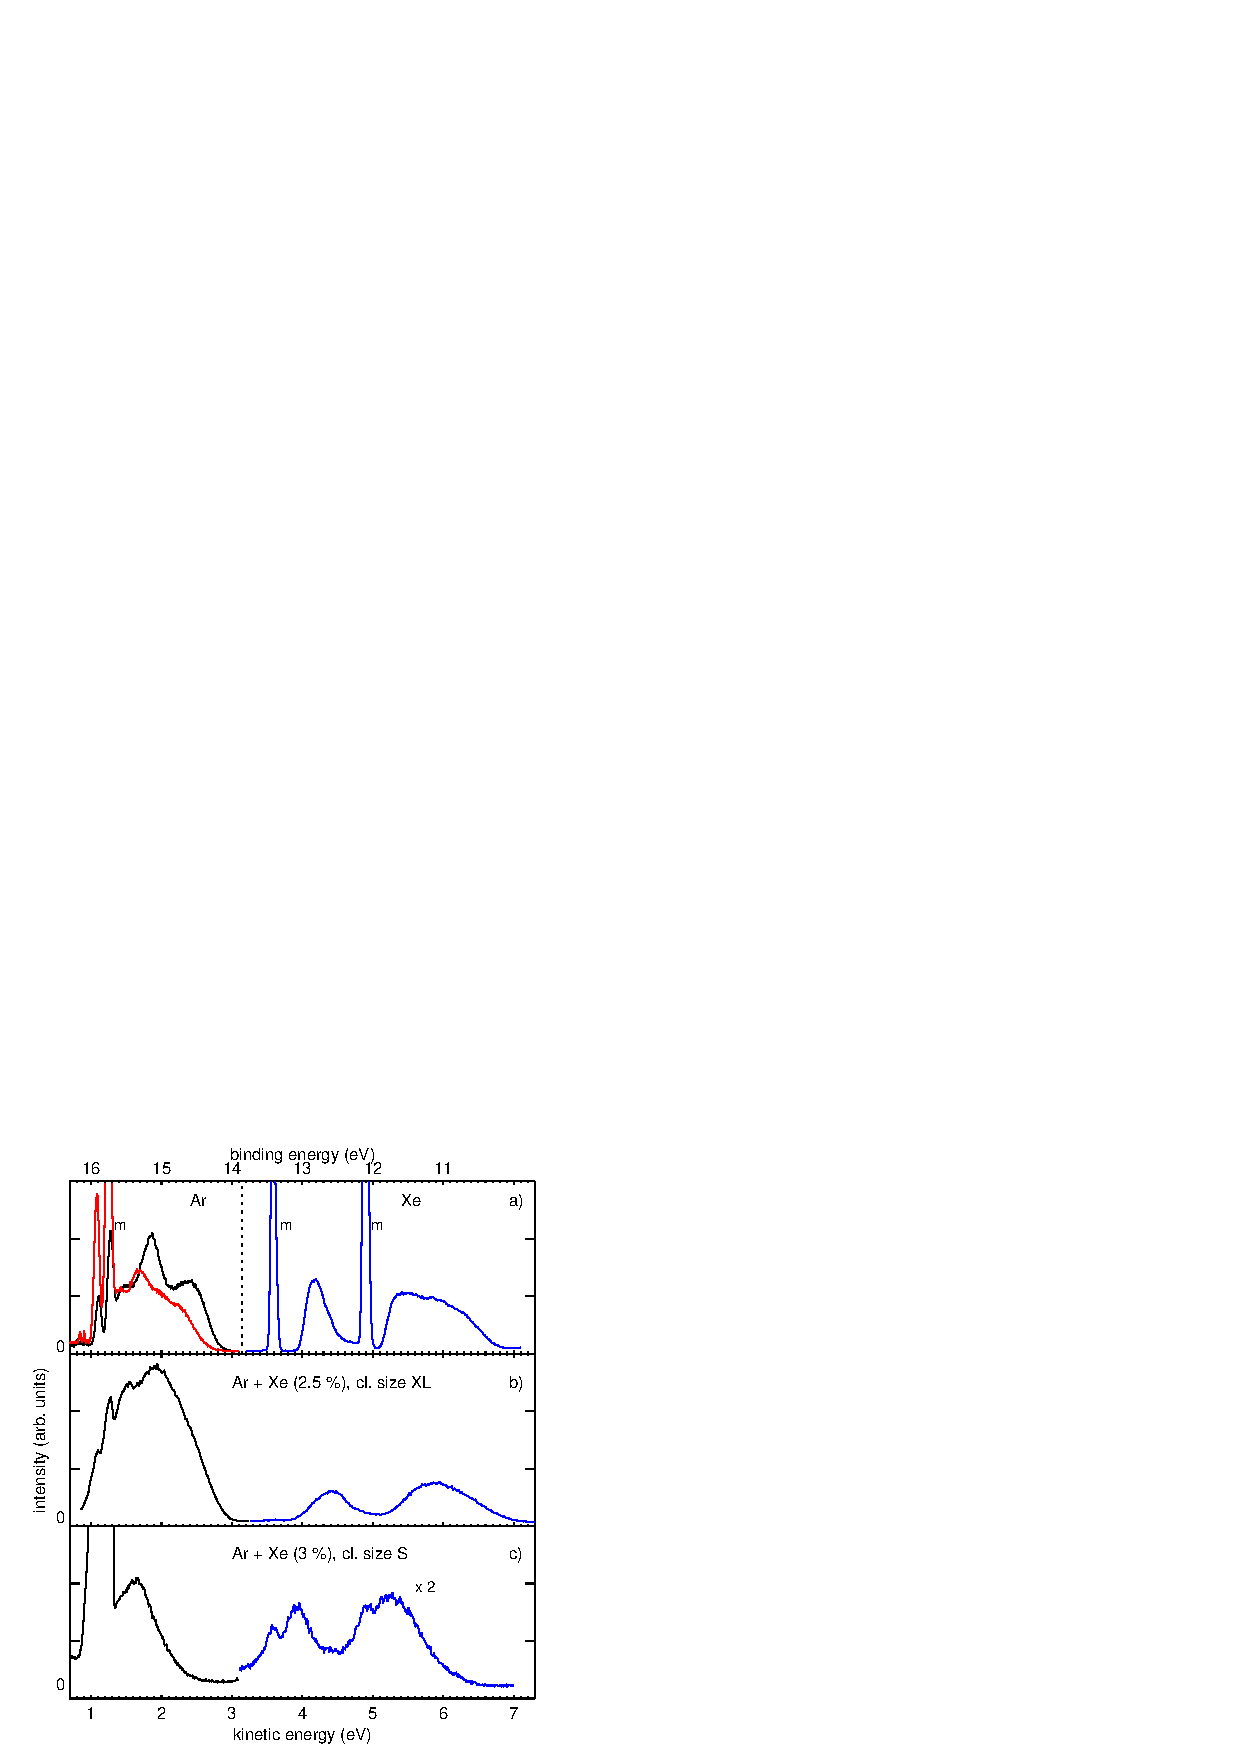
\includegraphics[width=8.5cm]{pics/figure_oval_1.pdf}
 \caption{
Outer valence photoelectron spectra of mixed Ar-Xe clusters, in comparison to the pure species. 
(a) shows the outer valence region of homogeneous Ar(1) (red) Ar(2) (black) and Xe clusters, respectively (see text and Table\ \ref{tab:cluster} for details). 
The two lower panels show spectra of the mixed species with different mean size. 
Sharp lines marked `m' (for `monomer') result from photoionization of uncondensed atoms into the Ar 3p$_{1/2,3/2}$ and Xe 5p$_{1/2,3/2}$ final states. 
Labels in (b) and (c) give the Xe content in the expanding gas mixture (Xe$_{\rm in}$), which is lower than the Xe content observed in the heterogeneous clusters (Xe$_{\rm cl}$). 
The photon energy was 17~eV, apart from the pure Xe cluster spectrum (60 eV).
%{\color{red}{Die Stabilisierung der Xe-bulk Atome ist in den gemischten Cluster
% höher als in den gemischten Clustern. Das ist ungewöhnlich. Habt ihr hier
% verschiedene CLustergrößen?}}
}
 \label{figure:oval1}
\end{figure}


\begin{figure}[ht]
 \centering
 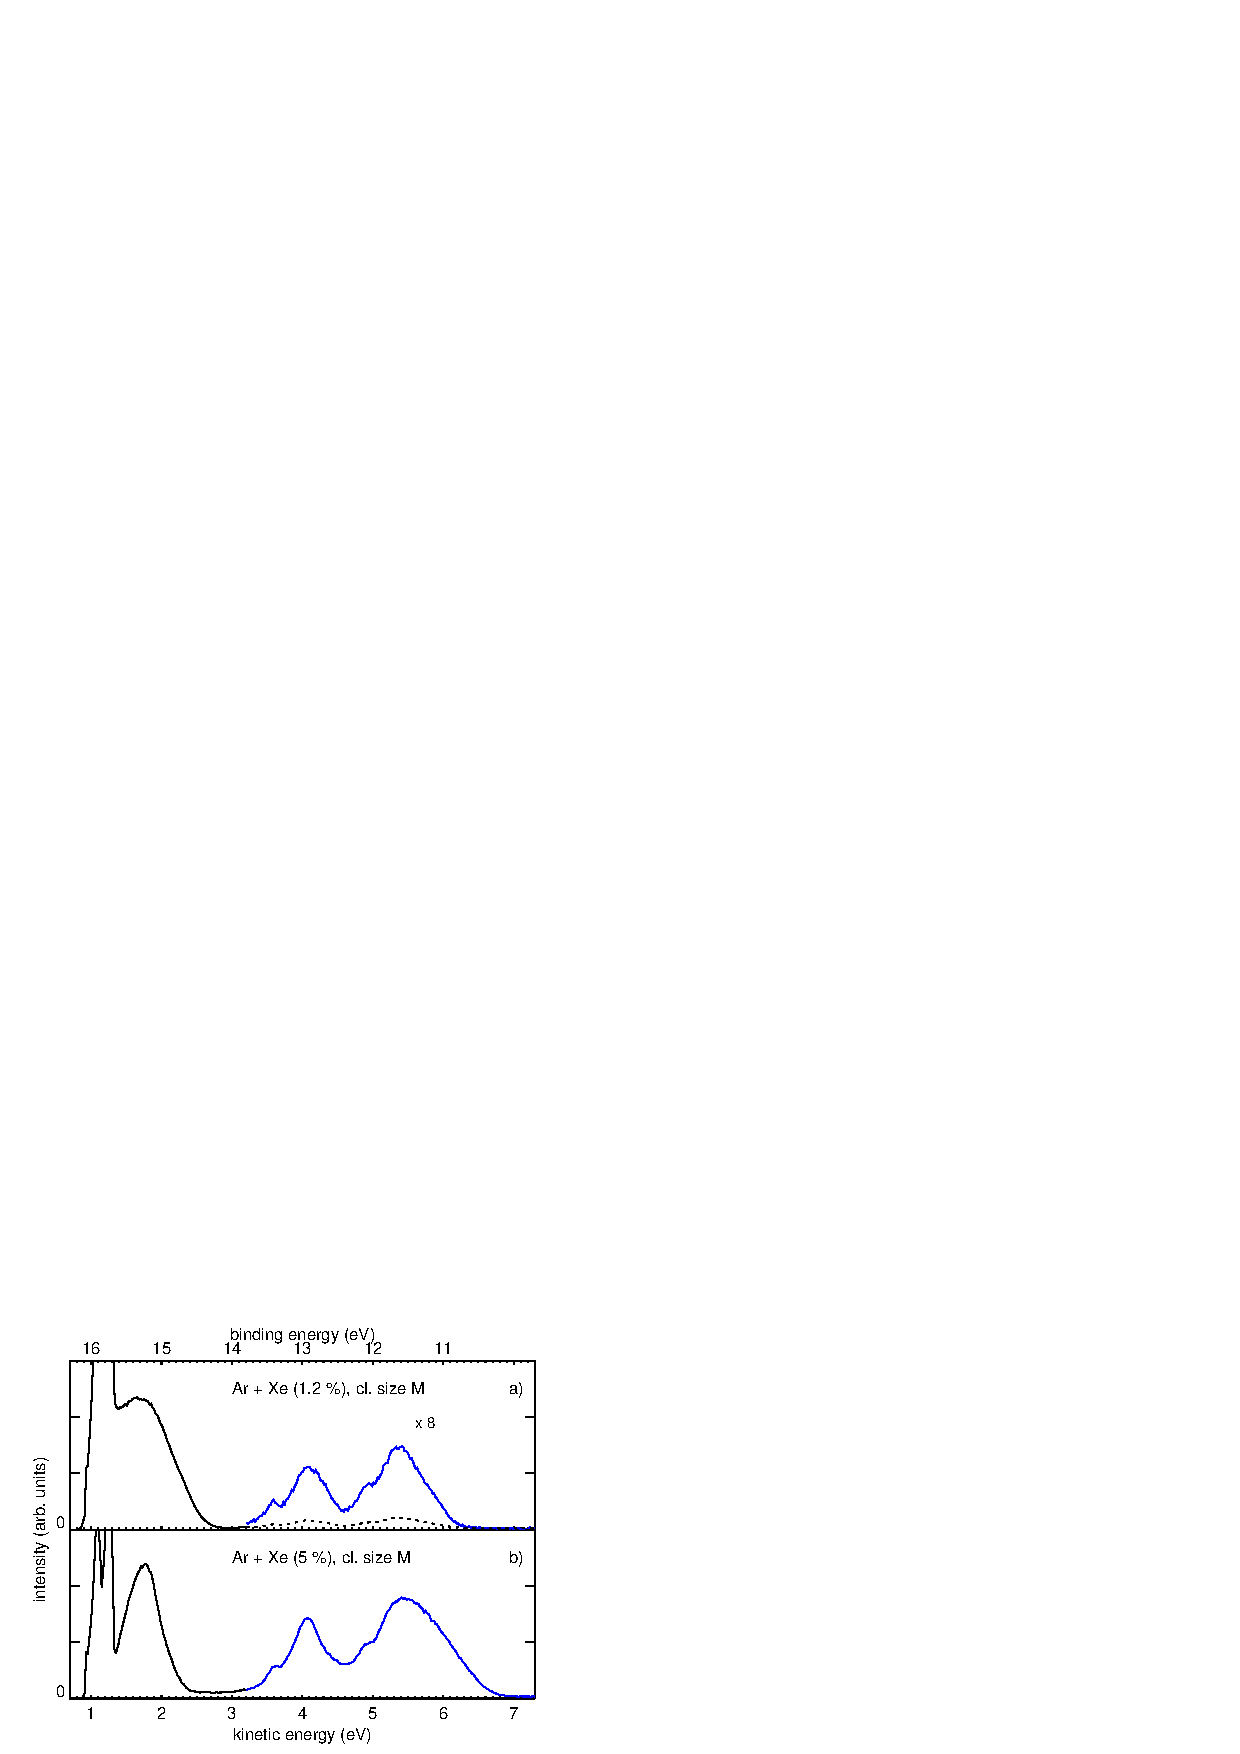
\includegraphics[width=8.5cm]{pics/figure_oval_2.pdf}
 \caption{
Outer valence photoelectron spectra of mixed Ar-Xe clusters from gas mixtures with different Xe concentration. 
For better visibility, a scaling factor is applied to the Xe part of the spectrum in panel (a). The dotted line shows the unscaled spectrum in this region.
See Figure \ref{figure:oval1} and text for details.
}
 \label{figure:oval2}
\end{figure}

Figure \ref{figure:oval1} shows the outer valence spectra of small and large ArXe clusters, compared to clusters of the pure gases. 
Qualitatively similar spectra have been published without detailed discussion in ref \citenum{lindblad}.
Differences are seen in particular for the Ar component. 
In pure Ar clusters, outer valence photoionization leads to a broad band, caused both by spin-orbit coupling and crystal field splitting. A distinction between the Ar 3p $_{1/2}$ and the Ar 3p $_{3/2}$ derived cluster bands can therefore not be made.
The relative importance of these two mechanisms remains under debate.\cite{hergenhahnprb,rolles,foerstel_arg1_2010}
For larger clusters (e.g. $\langle N\rangle = 190$, black trace), the maximum at low binding energies becomes more pronounced, and is identified with emission from the cluster interior.\cite{hergenhahnprb,rolles}
At the particular photon energy selected here, atop of this band a sharp feature is also visible (in Figure \ref{figure:oval1} at a kinetic energy of about 1.8 eV).
For larger clusters (above $\langle N\rangle \approx 100$), over a range of photon energies of about 3 eV, its appararent binding energy changes in a way which is reminiscent to photoemission of crystalline bulk matter (`dispersion').\cite{foerstel_arg1_2010,foerstel_arg2_2011} 

Ar 3p spectra of the smaller mixed clusters (Figure \ref{figure:oval1}c, Figure \ref{figure:oval2}) show neither of these traits.
Rather, the Ar band is symmetric, less wide than in the pure clusters and at a higher binding energy.
Even for very large clusters (Figure \ref{figure:oval1}b) the asymmetry of the 3p band and the `dispersing feature' do not appear.
We characterize the spectral shape by giving a single value for the Ar 3p binding energy, and the FWHM of the feature.
Values for different expansion parameters, and for both Ar and Xe valence lines, are collected in Table\ \ref{tab:valence}.

We find experimentally that clusters we have produced have a Xe content Xe$_{\rm cl}$ between 10\,\% and 50\,\%.
A slight decrease of the binding energy with cluster size is seen for all outer valence lines, and is attributed to a larger final state polarization energy in larger clusters. 

For further interpretation of the shape of the Ar peaks we refer to photoemission spectra of condensed Ar monolayers, measured in several settings.\cite{jacobi,jacobi2}
Spectra were reported for physisorption of Ar on two different metal single crystal substrates, and for Ar atop of a Xe spacer layer adsorbed on the metal.
While the binding energy depends on the substrate, the spectral shape is very similar in all cases. 
Most spectra were recorded for emission along the surface normal, and show a double peak split by about 0.5 eV, leading to a structure with $w$ about 1 eV.
Although the splitting is larger than the gas phase fine structure split of 0.18 eV, the pertaining states have been assigned to Ar 3p$_{1/2}$ and 3p$_{3/2}$.
A crystal field splitting of the 3p$_{3/2}$ state has been assumed to be also present, but with a smaller value of 0.1-0.2 eV, approx.\cite{jacobi2} 
The spectrum clearly changes when going to an emission angle of 40$^\circ$ with respect to the surface normal (Figure 2 in ref \citenum{jacobi2}).
The higher binding energy peak significantly loses in intensity, and the spectrum is now dominated by a single peak comprising both crystal field split substates of Ar 3p$_{3/2}$, with a FWHM ($w$) of only 0.4 eV.
As our measured spectrum is comprised of contributions recorded under all emission angles with respect to the cluster surface, grazing emission will be the rule.
We therefore believe that the arguments given above make it plausible that only a single peak is observed in all our spectra.

Emission from the Xe 5p state shows a much larger fine structure splitting then from the Ar 3p state; it dominates the spectrum even in clusters (where other broadening mechanisms are also present).
The shift of the cluster bands with respect to the monomer lines in the largest mixed clusters we have probed (Figure \ref{figure:oval1}b) are similar to the ones in the pure Xe spectrum, the scaling law size of which is at somewhat more than five filled shells.
This indicates an approximate upper limit for the size of the Xe core in our mixed clusters, as their binding energy shift might be somewhat higher than the one in pure clusters, due to polarization of covering Ar layers.
Xe cluster features in the spectra of mixed clusters appear less asymmetric than the pure Xe spectrum, and also less asymmetric as some the ArXe spectra shown in ref \citenum{lindblad}.
This might be caused by the difference in photon energy ($h\nu = 90$ eV in ref \citenum{lindblad} and for the pure Xe spectrum, $h\nu = 32$ eV for the mixed ArXe spectra in this work).
% For the mixed clusters, the Xe band broadens and shifts towards lower binding energy for larger size clusters.
%For pure Xe clusters, an asymmetry observed in the Xe 5p$_{3/2}$ part has no counterpart in the respective spectra from the mixed clusters.
%This might be caused by the difference in photon energy, as can be seen from a comparison to literature spectra (ArXe at $h\nu = 90$ eV in ref \citenum{lindblad}, Xe at $h\nu = 20$ eV in ref \citenum{rolles}).
%For the largest clusters, the nominal size yielded from the jet parameters applied to a pure Xe expansion would correspond to clusters in which bulk atoms far outweigh those on the surface.
%At least for the 5p$_{1/2}$ photoelectron line, this would be seen as a clear asymmetry towards the low binding energy side, which is not observed in our spectra.


In Figure \ref{figure:oval2}, we compare the outer valence spectra of clusters with similar expansion conditions, but different composition of the gas mixture.
A Xe-rich mixture obviously leads to clusters with more intense Xe photolines, but besides that the main change consists in a narrowing of the Ar band.
A comparison with the Ar monomer features (clipped in the Figure) also shows an increased degree of condensation for the Ar gas in the expansion.

For the smallest clusters we have produced, a possible model is provided by calculated minimum energy structures of Ar$_N$Xe$_{38-N}$ (Figure 7 in ref \citenum{marques}).
We there see that for a Xe content of less than 60\,\%, core-shell systems are {\it not} formed, and although the Xe atoms tend to connect, the degree of Ar-Xe mixing is large.
While for low Xe content (approx. 10\,\%), some Ar atoms have only Ar nearest neighbours, for larger Xe content all Ar atoms seem to see both Ar and Xe nearest neighbours.
We believe this leads to the Ar 3p narrowing pointed out above.
For Figure \ref{figure:oval2}, possibly, some clusters of our ensemble already are in the core-shell regime, which would lead to an even lower 3p width.

For the largest clusters we have produced (Figure \ref{figure:oval1}b), the low binding energy of the Xe lines and the broadening of the Ar feature without appearance of the `bulk Ar'-maximum, supports formation of a Xe core covered by at least two layers of Ar.
If the scaling law size for a pure Ar expansion is taken as the lower limit for the cluster size, from the observed Xe content we arrive at clusters composed of a Xe core with four layers, covered by three layers of Ar (see Supporting Information).

Finally, comparing Figure \ref{figure:oval2} to Figure \ref{figure:oval1} reveals that much larger changes in the valence emission spectra occur by changes in size than by changes of the (relative) Xe content.
This finding is supported by the spectra shown in ref \citenum{lindblad}.
%
%
\subsection{Inner valence spectra}
%
We now focus on the Ar inner valence (3s) vacancy states. 
%
\begin{figure}[ht]
 \centering
 \includegraphics[width=8.8cm]{pics/figure_ival.pdf}
 \caption{
Photon excited electron spectra of mixed Ar-Xe clusters in the inner valence region.
Symbols show the Ar 3s photoline from clusters (`cl') and uncondensed Ar monomers (`m'), atop of a background resulting from inelastic intracluster scattering of outer valence photoelectrons (`excitonic satellites').\protect\cite{hergenhahn2002}
The photon energy was $h\nu = 32$ eV.
Panel (a) shows all electrons accumulated.
For the same conditions, in panel (b) we only show electrons that were detected in coincidence with a secondary electron of lower kinetic energy.
The black solid trace in (a), and red solid trace in (b) result from a least squares fit to the cluster part of the spectrum. 
The red solid trace in (a) is the fit shown in (b), divided by the detection efficiency of the spectrometer of 0.6.
Panels (c) and (d) show the same type of data for smaller clusters with a lower Xe content.
See text for details.
\label{figure:ival}
}
\end{figure}

Figure\ \ref{figure:ival} shows the Ar part of the inner valence spectrum for representative ArXe clusters. 
The total photoelectron signal looks similar to literature spectra for pure Ar clusters.\cite{feifel,zhang} 
A low energy tail seen for the Ar 3s monomer line results from the transmission properties of the electron spectrometer, together with the strongly positive angular distribution parameter of this line.\cite{zhang,kruit}
The Ar 3s cluster line shows no splitting into bulk and surface components, different to the literature on pure clusters but in agreement with our discussion of the outer valence spectra. 
The binding energy of the cluster line has values between 28.85 and 28.70 eV for all cluster ensembles with size label S-L, and 28.67 eV for the largest clusters measured. 
A small, but systematic decrease of the binding energy is observed when the cluster size is increased. 
The value assumed in the simulations is 28.7 eV.

If we produce a spectrum only from those electrons recorded as part of a two-electron coincidence (electron pair with kinetic energies ($e_1,e_2$)) the apparent intensity drops (compare panel b to a, and d to c in Figure \ref{figure:ival}).
This can partly be attributed to the finite detection efficiency of the spectrometer. 
Moreover, the monomer part of the Ar 3s signal completely disappears, as 3s photoionization of an uncondensed Ar atom in the gas jet cannot lead to emission of a second electron. 
Further features of these diagrams and the least squares fits shown in the Figure are discussed below.
%
%
\subsection{ICD/ETMD spectra}
%
\begin{figure}[ht]
 \centering
 \includegraphics[width=8.5cm]{pics/figure_icd_12.pdf}
 \caption{
Energy spectrum of all coincident secondary (ICD or ETMD) electrons of kinetic energy $e_2$ pertaining to primary electrons of kinetic energy $e_1$ in the Ar 3s binding energy region. 
Spectra were recorded with a photon energy of $h\nu = 32$~eV. 
Black error bars show the data points for the smallest clusters measured (`S'), two larger clusters sizes are shown by the red and blue traces. 
Error bars for the latter are smaller than the ones shown and have been omitted.
For better comparison, all spectra are shown area-normalized. 
}
 \label{figure:icd_12}
\end{figure}
%
%
\begin{figure}[ht]
 \centering
 \includegraphics[width=8.5cm]{pics/figure_icd_l.pdf}
 \caption{
Energy spectrum of all coincident secondary (ICD or ETMD) electrons, kinetic energy $e_2$, for clusters of the same size, but from gas mixtures with different Xe concentration. See Figure \protect\ref{figure:icd_12} for details.
}
 \label{figure:icd_l}
\end{figure}
%
In Figure \ref{figure:icd_12}, we show the spectra of ICD/ETMD electrons pertaining to emission of an Ar 3s cluster photoelectron. 
Due to their low kinetic energy, without use of a coincidence method they could hardly be separated from the background of inelastically scattered photoelectrons.\cite{mucke}
This and the following Figure constitute the central experimental result of the article.
Spectra recorded at $h\nu = 34$ eV as a cross-check quantitatively agree to those shown here.
This underpins our assignment of this intensity to an autoionization process.
Further details on the data acquisition and analysis methodology, as well as the 34~eV spectra, are given in the Supporting Information.

Spectra for the three different cluster sizes in Figure \ref{figure:icd_12} are significantly different: Spectra for the larger clusters acquire more intensity in the 1-1.5 eV region and have less intensity for energies below 0.5 eV.
In contrast to that, the ICD/ETMD spectrum hardly varies when the composition of the expanding gas mixture, and with that the relative Xe content of the clusters, is changed (Figure \ref{figure:icd_l}).
The full set of ICD/ETMD spectra is shown as Supporting Information.

\begin{figure}[ht]
 \centering
 \includegraphics[width=8.5cm]{pics/figure_eff.pdf}
 \caption{
Efficiency of the decay of Ar 3s ionized states in ArXe clusters by emission of a secondary electron via ICD or ETMD. Values are arranged by Xe content of the initial gas mixture (`+' symbols: 1.2\,\%, asterisk: 3\,\%, triangle: 5\,\%). Symbol sizes indicate the photon energy (large symbols: 32 eV, small: 34 eV), and color indicates the cluster size (black symbols: S, red: M, blue: L). See text for details.
}
 \label{figure:eff}
\end{figure}
%
We now discuss which fraction of Ar 3s vacancy states relaxes via ICD or ETMD.
A method to derive this information has been established by some of us.\cite{foerstel_2013}
Briefly, we correct the intensity of the Ar 3s photoline in the coincident spectra by the detector efficiency, and divide it by the total (coincident and non-coincident) Ar 3s intensity.
The result gives the branching ratio of decay via ICD/ETMD vs. the sum of all channels, including those not involving electron emission.
(If all Ar 3s vacancies decay by emission of another electron, the coincident and non-coincident count rate differ only by the probability for the spectrometer to actually detect the secondary electron.
This figure has been determined as 0.6 for this data set, in the same way as discussed earlier.\cite{mucke_review})
To arrive at quantitative results, we have performed least squares fits of the non-coincident and coincident $e_1$ spectra.
The fits assumed one or two Gaussian peaks, resp., atop of a background modelled by two more Gaussian curves with very large widths.
The peak pertaining to the Ar 3s cluster photoline, with the background added, is shown by the black solid trace in Figure \ref{figure:ival}a and red solid trace in Figure \ref{figure:ival}b.
Moreover, the line labelled `c.fit/det.' shows the fit to the coincident events, corrected by the detection efficiency, and plotted atop of the non-coincident intensity. 
This virtually agrees with the fit to the total spectrum in Figure \ref{figure:ival}a, but not in \ref{figure:ival}c. 
The corresponding figure for the ICD/ETMD efficiency comes out as one for \ref{figure:ival}a, and significantly smaller than one for \ref{figure:ival}c.
Figure \ref{figure:eff} shows all results of this analysis.
The error in the autoionization efficiency shown is mainly determined by uncertainties in the peak/background separation.
%(Our choice for the background shape is shown in Figure \ref{figure:ival}.)
For the gas mixture with a Xe$_{\rm in}$ of 1.2\,\%, we therefore show results from fits using two different choices of the background shape in Figure \ref{figure:eff}.
Statistical errors are much smaller than the differences between the pairs of values arrived at such.

We found an Ar 3s autoionization efficiency which is compatible with unity, within the accuracy of our experiment, for all clusters except those with the lowest Xe content (Xe$_{\rm cl}$ approx. 10-12\,\%).
For the latter, also a decrease of the efficiency with decreasing cluster size is seen. 
Two main reasons can be identified that may cause a decrease in autoionization efficiency. 
Firstly, in small clusters with a low Xe content, for some Ar atoms no Xe partners allowing either ICD or ETMD might be available.
A simple example are clusters containing just a single Xe atom.
This mechanism would gain in importance for cluster ensembles with small $\langle N\rangle$.
Secondly, if only Xe partners at very large distances are available, ICD might be outpaced by other decay processes, most importantly fluorescence.


\section{Discussion
\label{sec:discussion}}
%
%We have discussed the experimental spectra in Section \ref{sec:exp_results} and
%the expected features of spectra for different cluster types in
%Section \ref{sec:th_results}. In this section we combine the experimental and theoretical
%results in order to determine the structure of the noble gas clusters.
%
%The simulated secondary electron spectra for the xenon core structures
%(see Figure \ref{figure:xe_3_in})
%show an ICD peak at higher energies than those structures with added xenon
%atoms on the surface. This does not fit to the experimentally determined
%spectra and hence we consider an argon core to be more probable for the
%small measured clusters.
%
%The experimental spectra in Figure \ref{}
%show a broadening of the secondary electron peak with increasing
%pressure (?) and hence cluster size just as can be expected from
%the theoretically simulated spectra in Figure \ref{figure:surf}.
%
%From the theoretical simulations of larger small clusters
%having the same xenon content as experimentally observed a clearly
%visible ETMD peak is to be expected as shown in Figure \ref{figure:ar_3_6in}.
%However, the experimental spectra do not show a signal in the energy
%region of \unit[1.5--6.5]{eV}. From this we conclude that the clusters
%measured were smaller than 55 atoms containing only very few xenon atoms.
%Additionally, if the cluster contains more than one xenon atom, they are
%not expected to be close because of an otherwise visible ETMD peak
%(compare Figure \ref{figure:2tops}).
%
%The large clusters with a large xenon content can be expected to have
%a xenon core being surrounded by argon layers and hence, both ICD and
%ETMD should be visible in the spectrum. Unfortunately, the ICD and ETMD
%peaks overlap such that the two processes can not be distiguished.
%
We now would like to interpret our experimental findings in view of the simulated results described in Section `Theoretical Results'.
Figure \ref{figure:eff} shows that for Ar 3s$^{-1}$ states autoionization by either ICD or ETMD is the only mode of relaxation, except for the clusters with the smallest Xe content.
We consider this a remarkable result, because ICD in this system is only possible with a Xe atom in the second coordination shell of the decaying Ar vacancy (or shells even further apart), which reduces its decay rate.
Also decay rates for ETMD were found to be small in early studies of this effect.\cite{zobeley}
Nevertheless, even in this situation the non-local autoionization channels foreclose radiative decay.

% lowest kinetic energy is the first point of energy raster for t-E code of 52-proc-spec
Structurally, all experimental ICD/ETMD spectra have a maximum at or near the lowest kinetic energy that could be measured (50~meV), and decrease in intensity to less than half for kinetic energies below one eV. 
Qualitatively, this shape fits to the ICD contributions in the autoionization spectra discussed in the `Theory' section, but not to the ones from ETMD. 
The calculated ETMD spectra have a typical three-fold structure with peaks between 3.5-5~eV, 1.5-2.5~eV and around 0 eV kinetic energy. 
The former two features seem not to be present in the experimental spectra. 
Due to restrictions in the detector electronics, electron pairs with very similar kinetic energy cannot be detected. 
The highest kinetic energy for an autoionization electron that can be detected in coincidence with a photoelectron of $\sim3.5$~eV ($h\nu = 32$~eV) is around 2.5~eV.
Very weak intensity is observed at this energy, and also at higher $e_2$ energies that can be probed at $h\nu = 34$~eV (Supporting Information).

As a cross-check for our theoretical methods we have calculated the radiationless decay spectrum of Ar 3s$^{-1}$ in ArKr, which may arise {\it only} from ETMD(3),\cite{foerstel} and arrived at qualitative agreement with the experimental data.\cite{arkr}

The size-dependent trend within the experimental data is in qualitative agreement to the change in the calculated spectral shape for ICD in systems of increased size (compare Figure~\ref{figure:2tops} to \ref{figure:xe_3_in} and \ref{figure:xe_6_lay5}.)

We are therefore lead to the conclusion that the autoionization spectra we incur are dominated by ICD to non-nearest neighbour atoms, while the intensity of the ETMD channel is low. 
We would like to recall the factors that lead to a propensity for decay via one or the other mechanism, which have been discussed in the `Theoretical Results'-section.
For ETMD to occur with a measurable rate, two Xe atoms have to be present in the vincinity of the decaying Ar atom (Figure \ref{figure:2tops}).
Should that be the case for a large part of the Ar atoms in some structure, ETMD can even dominate over ICD (Figure \ref{figure:ar_3_6in} and Supporting Information).
Model structures shown in Figures \ref{figure:2tops} and \ref{figure:ar_3_6in} have a Xe content similar to the lowest one probed in our experiment ($\sim$11\,\%).
For a higher Xe content, ETMD will always dominate the spectra if the two species are given the chance to mix, as e.g. in the calculated minimum energy structures of $N=38$ ArXe clusters (Supporting Info).
On the other hand, in core-shell systems decay via ETMD is probable only for Ar atoms in the interface layer, as this mechanism requires some wavefunction overlap between Ar and one of the Xe atoms involved.
For the core-shell systems we have investigated, the likelihood of decay via ETMD stays below 25\,\% even for a Xe content above 50\,\% (Table \ref{table:theo_gammas}).

In summary, the two structural motifes that can best be reconciled with our experimental data are
\begin{enumerate}
	\item small clusters containing only few Xe atoms that are spread out to distant positions on the cluster surface, and
	\item systems with a compact Xe core and Ar outer layers.
\end{enumerate}
These structures are compatible with the findings of Lindblad {\it et al.}\ from core level photoelectron spectroscopy, who proposed the former structure for the smallest clusters in their study, and the latter for larger ones.\cite{lindblad}
As even in these two cases intensity for decay via ETMD would not vanish completely, we have to leave it open though whether other mechanisms are present, which further suppress ETMD vs. ICD.

While in early work on ICD it has almost been a paradigm that the decay involves two {\it neighbouring} atoms or molecules,\cite{hergenhahn_review} more recently significant intensity for non-nearest neighbour ICD has been found also in other systems.
One example is Ne-Ar after Ne 2s ionization, where decay to Ar in the second coordination shell is clearly visible despite the fact that in this system decay involving nearest neighbours is energetically allowed.\cite{fasshauer2014}
A further theoretical delineation of the respective factors has recently been presented by onw of us.\cite{fasshauernjp}
%\section{Discussion of Experimental Results}

\section{Summary}
%
In summary, we have presented comprehensive experimental and theoretical data for the autoionization of inner valence ionized states in ArXe clusters.
Both ICD and ETMD are allowed for most cases we considered.
Because of energetical reasons ICD requires a separation of the final state vacancies by about 8~\AA or more, which is at least two times the typical Ar-Xe distance.
We found that autoionization has 0.8 to 1.0 efficiency within the experimental accuracy, that is it dominates over other modes of relaxation.
By comparing our measured spectra to calculations, we identified `long range' ICD as the most important decay mode.

%%%%%%%%%%%%%%%%%%%%%%%%%%%%%%%%%%%%%%%%%%%%%%%%%%%%%%%%%%%%%%%%%%%%%
%% The "Acknowledgement" section can be given in all manuscript
%% classes.  This should be given within the "acknowledgement"
%% environment, which will make the correct section or running title.
%%%%%%%%%%%%%%%%%%%%%%%%%%%%%%%%%%%%%%%%%%%%%%%%%%%%%%%%%%%%%%%%%%%%%
\begin{acknowledgement}
%
We thank HZB for the allocation of synchrotron radiation beamtime, and the Deutsche Forschungsgemeinschaft for funding via the Forschergruppe 1789.
%
\end{acknowledgement}


%%%%%%%%%%%%%%%%%%%%%%%%%%%%%%%%%%%%%%%%%%%%%%%%%%%%%%%%%%%%%%%%%%%%%
%% The same is true for Supporting Information, which should use the
%% suppinfo environment.
%%%%%%%%%%%%%%%%%%%%%%%%%%%%%%%%%%%%%%%%%%%%%%%%%%%%%%%%%%%%%%%%%%%%%
%\begin{suppinfo}

%This will usually read something like: ``Experimental procedures and
%characterization data for all new compounds. The class will
%automatically add a sentence pointing to the information on-line:

%\end{suppinfo}

%%%%%%%%%%%%%%%%%%%%%%%%%%%%%%%%%%%%%%%%%%%%%%%%%%%%%%%%%%%%%%%%%%%%%
%% The appropriate \bibliography command should be placed here.
%% Notice that the class file automatically sets \bibliographystyle
%% and also names the section correctly.
%%%%%%%%%%%%%%%%%%%%%%%%%%%%%%%%%%%%%%%%%%%%%%%%%%%%%%%%%%%%%%%%%%%%%
\bibliography{arxe}

\end{document}
